%%%%%%%%%%%%%%%%%%%%%%%%%%%%%%%%%%%%%%%%%%%%%%%%%%%%%%%%%%%%%%%%%%%%%%%%
% Beamer Presentation - LaTeX - Template Version 1.0 (10/11/12)
% This template has been downloaded from: http://www.LaTeXTemplates.com
% License: % CC BY-NC-SA 3.0 (http://creativecommons.org/)
% Modified by Rahmat M. Samik-Ibrahim

% REV386: Thu 28 Jul 2022 11:00
% REV375: Tue 15 Mar 2022 10:00
% REV372: Sun 06 Mar 2022 08:00
% REV370: Sun 20 Feb 2022 10:00
% REV363: Mon 20 Dec 2021 15:00
% STARTX: Wed 14 Sep 2016 10:00
%%%%%%%%%%%%%%%%%%%%%%%%%%%%%%%%%%%%%%%%%%%%%%%%%%%%%%%%%%%%%%%%%%%%%%%%%

% PACKAGES AND THEMES 
\documentclass[aspectratio=169, xcolor=table, notheorems, hyperref={pdfpagelabels=false}]{beamer}
%%%%%%%%%%%%%%%%%%%%%%%%%%%%%%%%%%%%%%%%%%%%%%%%%%%%%%%%%%%%%%%%%%%%%%%%
% Beamer Presentation - LaTeX - Template Version 1.0 (10/11/12)
% This template has been downloaded from: http://www.LaTeXTemplates.com
% License: % CC BY-NC-SA 3.0 (http://creativecommons.org/)
% Modified by Rahmat M. Samik-Ibrahim
% REV316 Wed 14 Jul 2021 13:42:41 WIB
% REV217 Tue Feb  4 15:10:30 WIB 2020
% REV198 Wed Mar 13 16:39:02 WIB 2019
% REV006 Mon Jan 22 19:10:41 WIB 2018
% REV005 Mon Oct  2 14:45:07 WIB 2017
% START  Thu Aug 25 14:15:19 WIB 2016
%%%%%%%%%%%%%%%%%%%%%%%%%%%%%%%%%%%%%%%%%%%%%%%%%%%%%%%%%%%%%%%%%%%%%%%%%

%% ZCZC NNNN
\newtheorem{example}{Example}

%%%%%%%%%%%%%%%%%%%%%%%%%%%%%%%%%%%%%%%%%%%%%%%%%%%%%%%%%%%%%%%%%%%%%%%%%

\let\Tiny=\tiny
\mode<presentation> {
% The Beamer class comes with a number of default slide themes
% which change the colors and layouts of slides. Below this is a list
% of all the themes, uncomment each in turn to see what they look like.
%\usetheme{Boadilla}
\usetheme{Madrid}
% ZCZC %%%%%%%%%%%%%%%%%%%%%%%%%%%%%%%%%%%%%%%%%%%%%%%%%%%%%%%%%%%%%%%%%%
% \usetheme{default} \usetheme{AnnArbor} \usetheme{Antibes} \usetheme{Bergen}
% \usetheme{Berkeley} \usetheme{Berlin} \usetheme{CambridgeUS} 
% \usetheme{Copenhagen} \usetheme{Darmstadt} \usetheme{Dresden}
% \usetheme{Frankfurt} \usetheme{Goettingen} \usetheme{Hannover}
% \usetheme{Ilmenau} \usetheme{JuanLesPins} \usetheme{Luebeck}
% \usetheme{Malmoe} \usetheme{Marburg} \usetheme{Montpellier}
% \usetheme{PaloAlto} \usetheme{Pittsburgh} \usetheme{Rochester}
% \usetheme{Singapore} \usetheme{Szeged} \usetheme{Warsaw}
% NNNN %%%%%%%%%%%%%%%%%%%%%%%%%%%%%%%%%%%%%%%%%%%%%%%%%%%%%%%%%%%%%%%%%%
% As well as themes, the Beamer class has a number of color themes
% for any slide theme. Uncomment each of these in turn to see how it
% changes the colors of your current slide theme.
%\usecolortheme{orchid}
%\usecolortheme{rose}
%\usecolortheme{seagull}
%\usecolortheme{seahorse}
\usecolortheme{whale}
% ZCZC %%%%%%%%%%%%%%%%%%%%%%%%%%%%%%%%%%%%%%%%%%%%%%%%%%%%%%%%%%%%%%%%%%
%\usecolortheme{albatross} \usecolortheme{beaver} \usecolortheme{beetle}
%\usecolortheme{crane} \usecolortheme{dolphin} \usecolortheme{dove}
%\usecolortheme{fly} \usecolortheme{lily} \usecolortheme{wolverine}
% NNNN %%%%%%%%%%%%%%%%%%%%%%%%%%%%%%%%%%%%%%%%%%%%%%%%%%%%%%%%%%%%%%%%%%
% To remove the footer line in all slides uncomment this line
%\setbeamertemplate{footline} 
% To replace the footer line in all slides uncomment this line
%\setbeamertemplate{footline}[page number] 
% To remove the navigation symbols from the bottom uncomment this line
\setbeamertemplate{navigation symbols}{} 
}

\usepackage{array}       % ZCZC
\usepackage{amssymb}     % ZCZC
\usepackage{bold-extra}  % ZCZC
\usepackage{booktabs}    % Allows \toprule, \midrule and \bottomrule in tables
\usepackage{caption}
\usepackage[T1]{fontenc} % ZCZC << >>
\usepackage{graphicx}    % Allows including images
\usepackage{listings}    % listing
\usepackage{lmodern}     % ZCZC
\usepackage{perpage}     % reset footnote per page
\usepackage{geometry}    % ZCZC
\usepackage{adjustbox}   % ZCZC
\usepackage{multirow}    % ZCZC

% \definecolor{links}{HTML}{2A1B81}
\definecolor{links}{HTML}{0011FF}
\hypersetup{colorlinks,linkcolor=,urlcolor=links}

% \usepackage{xcolor}
% \usepackage[colorlinks = true,
%             linkcolor = blue,
%             urlcolor  = blue,
%             citecolor = blue,
%             anchorcolor = blue]{hyperref}

\captionsetup[table]{name=Tabel}
\makeatletter
\def\input@path{{src/}}
\makeatother
\graphicspath{{src/}}      % src directory
\MakePerPage{footnote}     % reset page

% NNNN %%%%%%%%%%%%%%%%%%%%%%%%%%%%%%%%%%%%%%%%%%%%%%%%%%%%%%%%%%%%%%%%%%

%% % XXXXXXXXXXXXXXXXXXXXXXXXXXXXXXXXXXXXXXXXXXXXXXXXXXXXXXXXXXXXXXXXXXXXXXXXXX
%% % The short title appears at the bottom of every slide, 
%% % the full title is only on the title page
%% \title[Judul Pendek]{Judul Panjang dan Lengkap} 
%% \author{Cecak bin Kadal}
%% \institute[UILA]
%% {
%% University of Indonesia at Lenteng Agung \\ 
%% \medskip
%% \textit{cecak@binKadal.com}
%% }
%% \date{REV00 24-Aug-2016}
%% % \date{\today}
%% 

%% % XXXXXXXXXXXXXXXXXXXXXXXXXXXXXXXXXXXXXXXXXXXXXXXXXXXXXXXXXXXXXXXXXXXXXXXXXX
%% \begin{document}
%% \section{Judul}
%% \begin{frame}
%% \titlepage
%% \end{frame}
%% 
%% % XXXXXXXXXXXXXXXXXXXXXXXXXXXXXXXXXXXXXXXXXXXXXXXXXXXXXXXXXXXXXXXXXXXXXXXXXX
%% \section{Agenda}
%% \begin{frame}
%% \frametitle{Agenda}
%% % Throughout your presentation, if you choose to use \section{} and 
%% % \subsection{} commands, these will automatically be printed on 
%% % this slide as an overview of your presentation
%% \tableofcontents 
%% \end{frame}
%% 
%% % XXXXXXXXXXXXXXXXXXXXXXXXXXXXXXXXXXXXXXXXXXXXXXXXXXXXXXXXXXXXXXXXXXXXXXXXXX
%% \section{UUD dan Pancasila}
%% \subsection{UUD}
%% \begin{frame}
%% \frametitle{Pembukaan}
%% Bahwa sesungguhnya kemerdekaan itu ialah hak segala bangsa dan oleh 
%% sebab itu, maka penjajahan diatas dunia harus dihapuskan karena 
%% tidak sesuai dengan perikemanusiaan dan perikeadilan.
%% \\~\\
%% Atas berkat rahmat Allah Yang Maha Kuasa dan dengan didorongkan oleh 
%% keinginan luhur, supaya berkehidupan kebangsaan yang bebas, maka 
%% rakyat Indonesia menyatakan dengan ini kemerdekaannya.
%% \end{frame}
%% 
%% % XXXXXXXXXXXXXXXXXXXXXXXXXXXXXXXXXXXXXXXXXXXXXXXXXXXXXXXXXXXXXXXXXXXXXXXXXX
%% \begin{frame}
%% \frametitle{Alenia Ketiga}
%% Kemudian daripada itu untuk membentuk suatu pemerintah negara Indonesia 
%% yang melindungi segenap bangsa Indonesia dan seluruh tumpah darah Indonesia 
%% dan untuk memajukan kesejahteraan umum, mencerdaskan kehidupan bangsa, dan 
%% ikut melaksanakan ketertiban dunia yang berdasarkan kemerdekaan, perdamaian 
%% abadi dan keadilan sosial, maka disusunlah kemerdekaan kebangsaan Indonesia 
%% itu dalam suatu Undang-Undang Dasar negara Indonesia, yang terbentuk dalam 
%% suatu susunan negara Republik Indonesia yang berkedaulatan rakyat dengan 
%% berdasar kepada:
%% \begin{itemize}
%% \item Ketuhanan Yang Maha Esa,
%% \item kemanusiaan yang adil dan beradab,
%% \item persatuan Indonesia,
%% \item dan kerakyatan yang dipimpin oleh hikmat kebijaksanaan 
%%       dalam permusyawaratan/ perwakilan,
%% \item serta dengan mewujudkan suatu keadilan sosial bagi seluruh rakyat 
%%       Indonesia.
%% \end{itemize}
%% \end{frame}
%% 
%% % XXXXXXXXXXXXXXXXXXXXXXXXXXXXXXXXXXXXXXXXXXXXXXXXXXXXXXXXXXXXXXXXXXXXXXXXXX
%% \subsection{Pancasila}
%% \begin{frame}
%% \frametitle{Tujuh Kunci Pokok}
%% \begin{block}{Pertama - Kedua - Ketiga}
%% Indonesia ialah negara berdasarkan hukum.
%% Sistem konstitusional.
%% Kekuasaan negara tertinggi di tangan MPR.
%% \end{block}
%% 
%% \begin{block}{Keempat - Kelima}
%% Presiden adalah penyelenggara pemerintahan tertinggi di bawah MPR.
%% Adanya pengawasan DPR.
%% \end{block}
%% 
%% \begin{block}{Keenam}
%% Menteri negara adalah pembantu presiden dan tidak bertanggung jawab 
%% kepada DPR.
%% \end{block}
%% 
%% \begin{block}{Ketujuh}
%% Kekuasaan kepala negara tidak tak tebatas.
%% \end{block}
%% 
%% \end{frame}
%% 
%% % XXXXXXXXXXXXXXXXXXXXXXXXXXXXXXXXXXXXXXXXXXXXXXXXXXXXXXXXXXXXXXXXXXXXXXXXXX
%% \section{Rupa-rupa}
%% \subsection{Kolom}
%% \begin{frame}
%% \frametitle{Kolom}
%% % The "c" option specifies centered vertical alignment 
%% % while the "t" option is used for top vertical alignment
%% \begin{columns}[c] 
%% % Left column and width
%% \column{.45\textwidth} 
%% \textbf{Heading}
%% \begin{enumerate}
%% \item Satu-satu
%% \item Dua-dua
%% \item Tiga-tiga
%% \item Satu-dua-tiga
%% \end{enumerate}
%% 
%% % Right column and width
%% \column{.5\textwidth}
%% Satu-satu~\dots{} aku sayang ibu!
%% Dua-dua~\ldots{} juga sayang ayah!
%% Tiga-tiga~\ldots{} sayang adik kakak!
%% Satu-dua-tiga~\ldots{} sayang semuanya!
%% 
%% \end{columns}
%% \end{frame}
%% 
%% % XXXXXXXXXXXXXXXXXXXXXXXXXXXXXXXXXXXXXXXXXXXXXXXXXXXXXXXXXXXXXXXXXXXXXXXXXX
%% \subsection{Tabel}
%% \begin{frame}
%% \frametitle{Tabel}
%% \begin{table}
%% \begin{tabular}{l l l}
%% \toprule
%% \textbf{Nama} & \textbf{NPM} & \textbf{Tanggal Lahir}\\
%% \midrule
%% Cecak bin Kadal & 1234567890 & 1 Jan 2015 \\
%% Aneh bin Ajaib  & 0987654321 & 31 Des 2014 \\
%% \bottomrule
%% \end{tabular}
%% \caption{Keterangan Tabel}
%% \end{table}
%% \end{frame}
%% 
%% % XXXXXXXXXXXXXXXXXXXXXXXXXXXXXXXXXXXXXXXXXXXXXXXXXXXXXXXXXXXXXXXXXXXXXXXXXX
%% \subsection{Teori}
%% \begin{frame}
%% \frametitle{Teori}
%% \begin{theorem}[Teori Satu Batu]
%% $E = mc^2$
%% \end{theorem}
%% \end{frame}
%% 
%% % XXXXXXXXXXXXXXXXXXXXXXXXXXXXXXXXXXXXXXXXXXXXXXXXXXXXXXXXXXXXXXXXXXXXXXXXXX
%% \subsection{Verbatim}
%% % Need to use the fragile option when verbatim is used in the slide
%% \begin{frame}[fragile] 
%% \frametitle{Verbatim}
%% \begin{example}[Teori Satu Batu]
%% \begin{verbatim}
%% \begin{theorem}[Teori Satu Batu]
%% $E = mc^2$
%% \end{theorem}
%% \end{verbatim}
%% \end{example}
%% \end{frame}
%% 
%% % XXXXXXXXXXXXXXXXXXXXXXXXXXXXXXXXXXXXXXXXXXXXXXXXXXXXXXXXXXXXXXXXXXXXXXXXXX
%% \subsection{Gambar}
%% \begin{frame}
%% \frametitle{Gambar}
%% \begin{figure}
%% \includegraphics[width=0.5\linewidth]{2}
%% \caption{Ini Gambar JPG}
%% \end{figure}
%% \end{frame}
%% 
%% % XXXXXXXXXXXXXXXXXXXXXXXXXXXXXXXXXXXXXXXXXXXXXXXXXXXXXXXXXXXXXXXXXXXXXXXXXX
%% \subsection{Rujukan}
%% % Need to use the fragile option when verbatim is used in the slide
%% \begin{frame}[fragile] 
%% \frametitle{Rujukan dan Kutipan}
%% Contoh penggunaan \verb|\cite| ketika mengutip\cite{p1}.
%% Perhatian: Beamer tidak mengerti \verb|\BibTeX|~\ldots
%% \footnotesize{
%%   \begin{thebibliography}{99} 
%%   \bibitem[Smith, 2012]{p1} John Smith (2012)
%%      \newblock Katak dalam Tempurung
%%      \newblock \emph{Jurnal Kelapa dan Amfibi} 12(3), 45 -- 678.
%%   \end{thebibliography}
%% }
%% \end{frame}
%% 
%% % XXXXXXXXXXXXXXXXXXXXXXXXXXXXXXXXXXXXXXXXXXXXXXXXXXXXXXXXXXXXXXXXXXXXXXXXXX
%% \subsection{Selesai}
%% \begin{frame}
%% \Huge{\centerline{Selesai}}
%% \end{frame}
%% 
%% % XXXXXXXXXXXXXXXXXXXXXXXXXXXXXXXXXXXXXXXXXXXXXXXXXXXXXXXXXXXXXXXXXXXXXXXXXX
%% \end{document}

\newcommand{\revision}{REV392 30-Aug-2022}
% w! tmptmp
% REV392: Tue 30 Aug 2022 12:00
% REV389: Mon 15 Aug 2022 08:00
% REV379: Tue 17 May 2022 05:00
% REV359: Sat 30 Oct 2021 14:00
% REV339: Sat 04 Sep 2021 12:00
% STARTS: Wed 24 Aug 2016 19:00
%%%%%%%%%%%%%%%%%%%%%%%%%%%%%%%%%%%%%
\newcommand{\kopikopi}{\textcopyright{}2016-2022 CBKadal + VauLSMorg}



% XXXXXXXXXXXXXXXXXXXXXXXXXXXXXXXXXXXXXXXXXXXXXXXXXXXXXXXXXXXXXXXXXXXXXXXXXX
% The short title appears at the bottom of every slide, 
% the full title is only on the title page
% \date{\today}
\title[\kopikopi]
{CSGE602055 Operating Systems \\ 
CSF2600505 Sistem Operasi \\
Week 04:
Addressing, Shared Lib, \& Pointer}
\author{C. BinKadal}
\institute[SDN]
{
Sendirian Berhad\\
\medskip
\url{https://os.vlsm.org/Slides/os04.pdf}
\\ \texttt{Always check for the latest revision!}
}
\date{\revision}

% XXXXXXXXXXXXXXXXXXXXXXXXXXXXXXXXXXXXXXXXXXXXXXXXXXXXXXXXXXXXXXXXXXXXXXXXXX
\begin{document}

\lstset{
basicstyle=\ttfamily\tiny, % \tiny \small \footnotesize 
breakatwhitespace=true,
language=C,
columns=fullflexible,
keepspaces=true,
breaklines=true,
tabsize=3, 
showstringspaces=false,
extendedchars=true}

\section{Start}
\begin{frame}
\titlepage
\end{frame}

% XXXXXXXXXXXXXXXXXXXXXXXXXXXXXXXXXXXXXXXXXXXXXXXXXXXXXXXXXXXXXXXXXXXXXXXXXX

%%%%%%%%%%%%%%%%%%%%%%%%%%%%%%%%%%%%%%%%%%%%%%%%%%%%%%%%%%%%%%%%%%%%%%%%%
% REV352 Sun 10 Oct 2021 09:56:47 WIB
% REV341 Sun 05 Sep 2021 23:30:00 WIB
% REV333 Thu 26 Aug 2021 08:52:24 WIB
% REV328 Sat 14 Aug 2021 06:32:08 WIB
% REV272 Mon 01 Mar 2021 12:02:09 WIB
% START0 Sat Sep  2 10:51:33 WIB 2017
%%%%%%%%%%%%%%%%%%%%%%%%%%%%%%%%%%%%%%%%%%%%%%%%%%%%%%%%%%%%%%%%%%%%%%%%%

\begin{frame}[fragile]
\section{Schedule}
\frametitle{OS212\footnote{%
) This information will be on \textbf{EVERY} page two (2) of this course material.}): 
Operating Systems 2021 - 2}
\scalebox{0.73}{%
\begin{tabular}{|c|c|c|c|}
\hline
\makebox[106pt]{OS A} & \makebox[106pt]{OS B} & \makebox[107pt]{OS C} & \makebox[107pt]{OS INT} \\
\hline
\multicolumn{4}{|c|}{Every first day of the Week, \textbf{Quiz\#1:} (07:40-07:50) and \textbf{Quiz\#2:} 07:20-07:40} \\
\hline
Monday/Thursday & Monday/Thursday & Monday/Thursday & Monday/Wednesday   \\
13:00 --- 14:40  & 15:00 --- 16:40\footnote{) \textbf{OS B:} Week00-Week05 (RMS); Week06-Week10 (MAM).} &
                                      13:00 --- 14:40 & 08:00 --- 09:40  \\
14:00 --- finish & 16:00 --- finish & 13:00 --- 14:40 & 09:00 --- finish \\
\hline
\end{tabular}
}

\vspace{5pt}

\scalebox{0.73}{%
\begin{tabular}{|c|c|l|l|}
\hline
\textbf{Week} & \textbf{Schedule \& Deadline}\footnote{%
    ) The \textbf{DEADLINE} of Week 00 is 05 Sep 2021,
      whereas the \textbf{DEADLINE} of Week 01 is 12 Sep 2021, and so on...%
    })& \textbf{Topic} & \textbf{OSC10}\footnote{%
    ) Silberschatz et. al.: \textbf{Operating System Concepts}, $10^{th}$ Edition, 2018.}) \\
\hline
Week 00  & 30 Aug - 05 Sep 2021 & Overview 1, Virtualization \& Scripting & Ch. 1, 2, 18. \\
Week 01  & 06 Sep - 12 Sep 2021 & Overview 2, Virtualization \& Scripting & Ch. 1, 2, 18. \\
Week 02  & 13 Sep - 19 Sep 2021 & Security, Protection, Privacy, \& C-language.  & Ch. 16, 17. \\
Week 03  & 20 Sep - 26 Sep 2021 & File System \& FUSE  & Ch. 13, 14, 15. \\
Week 04  & 27 Sep - 03 Oct 2021 & Addressing, Shared Lib, \& Pointer & Ch. 9. \\
Week 05  & 04 Oct - 10 Oct 2021 & Virtual Memory & Ch. 10. \\
\hline
Week 06  & 11 Oct - 31 Oct 2021 & Concurrency: Processes \& Threads & Ch. 3, 4. \\
Week 07  & 01 Nov - 07 Nov 2021 & Synchronization \& Deadlock & Ch. 6, 7, 8. \\
Week 08  & 08 Nov - 14 Nov 2021 & Scheduling + W06/W07 & Ch. 5. \\
Week 09  & 15 Nov - 21 Nov 2021 & Storage, Firmware, Bootloader, \& Systemd & Ch. 11. \\
Week 10  & 22 Nov - 28 Nov 2021 & I/O \& Programming & Ch. 12. \\%
% MidTerm  & 00 XXX 2020 (XX:XX-XX:XX) & MidTerm (UTS) & \cellcolor{red!44} TBA! \\
% Reserved & 00 XXX - 00 XXX 2020 & Q \& A & \\
% Final    & 00 XXX 2020 XX:XX & First Part Final  (UAS tahap I)  & \cellcolor{red!44} This schedule is   \\
% Extra    & NA & No Extra assignment & \cellcolor{red!44} subject to change. \\
\hline
\end{tabular}
}
\end{frame}

\begin{frame}[fragile]
\frametitle{\textbf{STARTING POINT} --- 
{
\definecolor{links}{HTML}{FDEE00}
\hypersetup{colorlinks,linkcolor=,urlcolor=links}
\url{https://os.vlsm.org/}
}
}
\begin{itemize}
\item[$\square$] \textbf{Text Book} ---
                 Any recent/decent OS book. Eg. (\textbf{OSC10}) Silberschatz et. al.: 
                 \textbf{Operating System Concepts}, $10^{th}$ Edition, 2018.
                 See also \url{https://www.os-book.com/OS10/}.
\item[$\square$] \textbf{Resources}
\begin{itemize}
\item[$\square$] \href{https://scele.cs.ui.ac.id/course/view.php?id=3268}{\textbf{SCELE OS212}} ---
\url{https://scele.cs.ui.ac.id/course/view.php?id=3268}.\\
The enrollment key is \textbf{XXX}.
\item[$\square$] \textbf{Download Slides and Demos from GitHub.com} \\
\url{https://github.com/UI-FASILKOM-OS/SistemOperasi/}:

                 {\scriptsize%
                 \href{https://os.vlsm.org/Slides/os00.pdf}{\texttt{os00.pdf} (W00)},
                 \href{https://os.vlsm.org/Slides/os01.pdf}{\texttt{os01.pdf} (W01)},
                 \href{https://os.vlsm.org/Slides/os02.pdf}{\texttt{os02.pdf} (W02)},
                 \href{https://os.vlsm.org/Slides/os03.pdf}{\texttt{os03.pdf} (W03)},

                 \href{https://os.vlsm.org/Slides/os04.pdf}{\texttt{os04.pdf} (W04)},
                 \href{https://os.vlsm.org/Slides/os05.pdf}{\texttt{os05.pdf} (W05)},
                 \href{https://os.vlsm.org/Slides/os06.pdf}{\texttt{os06.pdf} (W06)},
                 \href{https://os.vlsm.org/Slides/os07.pdf}{\texttt{os07.pdf} (W07)},

                 \href{https://os.vlsm.org/Slides/os08.pdf}{\texttt{os08.pdf} (W08)},
                 \href{https://os.vlsm.org/Slides/os09.pdf}{\texttt{os09.pdf} (W09)},
                 \href{https://os.vlsm.org/Slides/os10.pdf}{\texttt{os10.pdf} (W10)}.
                 }
\item[$\square$] \textbf{Problems}\\
                 {\scriptsize% 
                 \href{https://rms46.vlsm.org/2/195.pdf}{\texttt{195.pdf} (W00)},
                 \href{https://rms46.vlsm.org/2/196.pdf}{\texttt{196.pdf} (W01)},
                 \href{https://rms46.vlsm.org/2/197.pdf}{\texttt{197.pdf} (W02)},
                 \href{https://rms46.vlsm.org/2/198.pdf}{\texttt{198.pdf} (W03)},\\
                 \href{https://rms46.vlsm.org/2/199.pdf}{\texttt{199.pdf} (W04)},
                 \href{https://rms46.vlsm.org/2/200.pdf}{\texttt{200.pdf} (W05)},
                 \href{https://rms46.vlsm.org/2/201.pdf}{\texttt{201.pdf} (W06)},
                 \href{https://rms46.vlsm.org/2/202.pdf}{\texttt{202.pdf} (W07)},\\
                 \href{https://rms46.vlsm.org/2/203.pdf}{\texttt{203.pdf} (W08)},
                 \href{https://rms46.vlsm.org/2/204.pdf}{\texttt{204.pdf} (W09)},
                 \href{https://rms46.vlsm.org/2/205.pdf}{\texttt{205.pdf} (W10)}.}
\item[$\square$] \textbf{LFS} --- \url{http://www.linuxfromscratch.org/lfs/view/stable/}
\item[$\square$] \textbf{OSP4DISS} --- \url{https://osp4diss.vlsm.org/}
\item[$\square$] \textbf{DOIT} --- \url{https://doit.vlsm.org/001.html}
\end{itemize}
\end{itemize}
\end{frame}



% XXXXXXXXXXXXXXXXXXXXXXXXXXXXXXXXXXXXXXXXXXXXXXXXXXXXXXXXXXXXXXXXXXXXXXXXXX
% Throughout your presentation, if you choose to use \section{} and 
% \subsection{} commands, these will automatically be printed on 
% this slide as an overview of your presentation
\section{Agenda}
\begin{frame}{Outline}
  \frametitle{Agenda}
  \tableofcontents[sections={1-13}]
\end{frame}
\begin{frame}
   \frametitle{Agenda (2)}
   \tableofcontents[sections={14-}]
\end{frame}

% XXXXXXXXXXXXXXXXXXXXXXXXXXXXXXXXXXXXXXXXXXXXXXXXXXXXXXXXXXXXXXXXXXXXXXXXXX

%%%%%%%%%%%%%%%%%%%%%%%%%%%%%%%%%%%%%%%%%%%%%%%%%%%%%%%%%%%%%%%%%%%%%%%%%
% REV349 Sun 26 Sep 2021 09:13:27 WIB
% REV154 Thu Aug 23 11:22:02 WIB 2018
% START0 Thu Jul 26 20:01:45 WIB 2018
%%%%%%%%%%%%%%%%%%%%%%%%%%%%%%%%%%%%%%%%%%%%%%%%%%%%%%%%%%%%%%%%%%%%%%%%%

\section{Week 04: Topics}
\begin{frame}[fragile]
\frametitle{Week 04 Addressing:
Topics\footnote{Source: ACM IEEE CS Curricula 2013}}

\begin{itemize}
\item Bits, bytes, and words
\item Numeric data representation and number bases
\item Representation of records and arrays
\end{itemize}
\end{frame}


\begin{frame}[fragile]
\frametitle{Week 04 Addressing:
Learning Outcomes\footnote{Source: ACM IEEE CS Curricula 2013}}
\begin{itemize}
\item Explain why everything is data, including instructions, in computers. [Familiarity]
\item Explain the reasons for using alternative formats to represent numerical data. [Familiarity]
\item Describe the internal representation of non-numeric data, such as characters, strings, records, and arrays.  [Familiarity]
\end{itemize}

\end{frame}



% XXXXXXXXXXXXXXXXXXXXXXXXXXXXXXXXXXXXXXXXXXXXXXXXXXXXXXXXXXXXXXXXXXXXXXXXXX
\section{OSC10 (Silberschatz) Chapter 9: Main Memory}
\begin{frame}
\frametitle{OSC10 (Silberschatz) Chapter 9: Main Memory}
  \begin{itemize}
  \item OSC10 Chapter 9: Main Memory
  \begin{itemize}
  \item Background
  \item Contiguous Memory Allocation
  \item Paging
  \item Structure of the Page Table
  \item Swapping
  \item Example: The Intel 32 and 64-bit Architectures
  \item Example: ARMv8 Architecture
  \end{itemize}
  \end{itemize}
  \vfill \null
\end{frame}

% 8 XXXXXXXXXXXXXXXXXXXXXXXXXXXXXXXXXXXXXXXXXXXXXXXXXXXXXXXXXXXXXXXXXXXXXXXX
\section{Week 04: Addressing, Shared Lib, \& Pointer}
\begin{frame}
\frametitle{Week 04: Addressing, Shared Lib, \& Pointer}
\begin{itemize}
\item This will be a difficult week
\begin{itemize}
\item Pray! Pray! We got to pray just to make it today (McH)!
\item Turn To Page 394 (HP3)!
\end{itemize}
\item Hardware Address Protection
\item Binding \& Linking
\begin{itemize}
\item Address Binding
\item Address Space: Logical \& Physical
\item Dynamic \& Static Linking
\item MMU: Memory Management Unit
\item Base and Limit Registers
\item Swapping
\item Mobile Systems Problem: no swap
\end{itemize}
\item Memory Allocation
\begin{itemize}
\item Contiguous Allocation
\item Multiple-variable-partition Allocation
\item First, Best, Worst Fit Allocation Strategy
\end{itemize}
\item Fragmentation: External / Internal / Compaction
\end{itemize}
\end{frame}

% XXXXXXXXXXXXXXXXXXXXXXXXXXXXXXXXXXXXXXXXXXXXXXXXXXXXXXXXXXXXXXXXXXXXXXXXXX
\section{Paging}
\begin{frame}
\frametitle{Paging}
\begin{itemize}
\item Logical/Virtual Address
\begin{itemize}
\item Logical Memory Blocks: Pages
\item Page Number + Page Offset
\end{itemize}
\item Page Table
\begin{itemize}
\item Page number index $\Rightarrow$ frame number
\item PTE: Page Table Entry
\item Page Flags: Valid/ Invalid
\item TLB: Translation Look-aside Buffer (Associative Memory).
\item Two-Level Page-Table Scheme
\begin{itemize}
\item OPT: Outer Page Table (P1)
\item PT: Page Table (P2)
\end{itemize}
\item Three-Level Page-Table Scheme
\item Hashed Page Tables
\item Inverted Page Table
\end{itemize}
\item Physical Address
\begin{itemize}
\item Physical Memory Blocks: Frames
\item Offset (D)
\item Hierarchical Page Tables
\end{itemize}
\end{itemize}
\end{frame}

% XXXXXXXXXXXXXXXXXXXXXXXXXXXXXXXXXXXXXXXXXXXXXXXXXXXXXXXXXXXXXXXXXXXXXXXXXX
\section{Addressing}
\begin{frame}
\frametitle{Addressing (Eg. 16 bits)}

\begin{minipage}[t]{95mm}

\scalebox{0.52}{
\begin{tabular}{| c  |  c |  c |  c |  c |  c |  c |  c |  c |  c |  c |  c |  c |  c |  c |  c |  c |||c|c|c|c|}
\hline
\multicolumn{17}{| c |||}{}                                    & \multicolumn{4}{| c |}{}         \\
\multicolumn{17}{| c |||}{16 Bits Logical Address Table (HEX)} & \multicolumn{4}{| c |}{Examples} \\
\multicolumn{17}{| c |||}{}                                    & \multicolumn{4}{| c |}{}         \\
\hline
     &    &    &    &    &    &    &    &    &    &    &    &    &    &    &    &    &      &     &     &       \\
ADDR &  0 &  1 &  2 &  3 &  4 &  5 &  6 &  7 &  8 &  9 &  A &  B &  C &  D &  E &  F & bits & L/B & PTR & VALUE \\
     &    &    &    &    &    &    &    &    &    &    &    &    &    &    &    &    &      &     &     &       \\
\hline
\hline
     &    &    &    &    &    &    &    &    &    &    &    &    &    &    &    &    &      &     &     &       \\
000X & A0 & A1 & A2 & A3 & A4 & A5 & A6 & A7 & A8 & A9 & AA & AB & AC & AD & AE & AF & 8    &
                                                                            --- & \textbf{[0008]} & \textbf{A8} \\
     &    &    &    &    &    &    &    &    &    &    &    &    &    &    &    &    &      &     &     &       \\
\hline
     &    &    &    &    &    &    &    &    &    &    &    &    &    &    &    &    &      &     &     &       \\
001X & B0 & B1 & B2 & B3 & B4 & B5 & B6 & B7 & B8 & B9 & BA & BB & BC & BD & BE & BF & 8    &
                                                                            --- & \textbf{[0014]} & \textbf{B4} \\
     &    &    &    &    &    &    &    &    &    &    &    &    &    &    &    &    &      &     &     &       \\
\hline
     &    &    &    &    &    &    &    &    &    &    &    &    &    &    &    &    &      &     &     &       \\
002X & C0 & C1 & C2 & C3 & C4 & C5 & C6 & C7 & C8 & C9 & CA & CB & CC & CD & CE & CF & 8    & --- &
                                                                                  \textbf{[0015]} & \textbf{B5} \\
     &    &    &    &    &    &    &    &    &    &    &    &    &    &    &    &    &      &     &     &       \\
\hline
     &    &    &    &    &    &    &    &    &    &    &    &    &    &    &    &    &      &     &     &       \\
003X & D0 & D1 & D2 & D3 & D4 & D5 & D6 & D7 & D8 & D9 & DA & DB & DC & DD & DE & DF & 16   & LE  &
                                                                        \textbf{[0014]}     & \textbf{B5 B4}    \\
     &    &    &    &    &    &    &    &    &    &    &    &    &    &    &    &    &      &     &     &       \\
\hline
     &    &    &    &    &    &    &    &    &    &    &    &    &    &    &    &    &      &     &     &       \\
004X & 0A &    &    &    &    &    &    &    &    &    &    &    &    &    &    &    & 16   & BE  &
                                                                        \textbf{[0014]}     & \textbf{B4 B5}    \\
     &    &    &    &    &    &    &    &    &    &    &    &    &    &    &    &    &      &     &     &       \\
\hline
     &    &    &    &    &    &    &    &    &    &    &    &    &    &    &    &    &      &     &     &       \\
\vdots & \vdots & \vdots & \vdots & \vdots & \vdots & \vdots & \vdots & \vdots & \vdots & \vdots & \vdots & 
\vdots & \vdots & \vdots & \vdots & \vdots & 32     & LE     & \textbf{[0014]}     & \textbf{B7 B6 B5 B4} \\
     &  &    &    &    &    &    &    &    &    &    &    &    &    &    &    &    &      &     &     &       \\
\hline
     &    &    &    &    &    &    &    &    &    &    &    &    &    &    &    &    & 
                                                                     \multicolumn{4}{| l |}{1 address == 1 byte} \\
FFFX &    &    &    &    &    &    &    &    &    &    &    &    &    &    &    &    &
                                                                     \multicolumn{4}{| l |}{LE: Little Endian}   \\
     &    &    &    &    &    &    &    &    &    &    &    &    &    &    &    &    & 
                                                                     \multicolumn{4}{| l |}{BE: Big Endian}      \\
\hline
\end{tabular}}
\end{minipage}
\\[1mm]

\end{frame}

% XXXXXXXXXXXXXXXXXXXXXXXXXXXXXXXXXXXXXXXXXXXXXXXXXXXXXXXXXXXXXXXXXXXXXXXXXX
\section{Translation}
\begin{frame}[fragile]
\frametitle{Address Translation Scheme}
\begin{minipage}[t]{120mm}
\centering
\scalebox{0.44}{
\begin{tabular}
{| c   | c    ||| c       || c   | c    || c   | c    || c   | c    || c    | c   |}
\hline
\multicolumn{2}{|c|||}{Address} &  \multicolumn{9}{|c|}{Binary}  \\
\hline
   DEC  & HEX  &   OFFSET  &  PG  & OFF  &  PG  & OFF  &  PAGE & OFF &  PAGE &  OFF   \\
\hline
   00   & 00   &   00000   &  0   & 0000 &  00  & 000  &  000 & 00   &  0000 &  0   \\
\hline
   01   & 01   &   00001   &  0   & 0001 &  00  & 001  &  000 & 01   &  0000 &  1   \\
\hline
   02   & 02   &   00010   &  0   & 0010 &  00  & 010  &  000 & 10   &  0001 &  0   \\
\hline
   03   & 03   &   00011   &  0   & 0011 &  00  & 011  &  000 & 11   &  0001 &  1   \\
\hline
   04   & 04   &   00100   &  0   & 0100 &  00  & 100  &  001 & 00   &  0010 &  0   \\
\hline
   05   & 05   &   00101   &  0   & 0101 &  00  & 101  &  001 & 01   &  0010 &  1   \\
\hline
   06   & 06   &   00110   &  0   & 0110 &  00  & 110  &  001 & 10   &  0011 &  0   \\
\hline
   07   & 07   &   00111   &  0   & 0111 &  00  & 111  &  001 & 11   &  0011 &  1   \\
\hline
\hline
   08   & 08   &   01000   &  0   & 1000 &  01  & 000  &  010 & 00   &  0100 &  0   \\
\hline
   09   & 09   &   01001   &  0   & 1001 &  01  & 001  &  010 & 01   &  0100 &  1   \\
\hline
   10   & 0A   &   01010   &  0   & 1010 &  01  & 010  &  010 & 10   &  0101 &  0   \\
\hline
   11   & 0B   &   01011   &  0   & 1011 &  01  & 011  &  010 & 11   &  0101 &  1   \\
\hline
   12   & 0C   &   01100   &  0   & 1100 &  01  & 100  &  011 & 00   &  0110 &  0   \\
\hline
   13   & 0D   &   01101   &  0   & 1101 &  01  & 101  &  011 & 01   &  0110 &  1   \\
\hline
   14   & 0E   &   01110   &  0   & 1110 &  01  & 110  &  011 & 10   &  0111 &  0   \\
\hline
   15   & 0F   &   01111   &  0   & 1111 &  01  & 111  &  011 & 11   &  0111 &  1   \\
\hline
\hline
\hline
   16   & 10   &   10000   &  1   & 0000 &  10  & 000  &  100 & 00   &  1000 &  0   \\
\hline
   17   & 11   &   10001   &  1   & 0001 &  10  & 001  &  100 & 01   &  1000 &  1   \\
\hline
   18   & 12   &   10010   &  1   & 0010 &  10  & 010  &  100 & 10   &  1001 &  0   \\
\hline
   19   & 13   &   10011   &  1   & 0011 &  10  & 011  &  100 & 11   &  1001 &  1   \\
\hline
   20   & 14   &   10100   &  1   & 0100 &  10  & 100  &  101 & 00   &  1010 &  0   \\
\hline
   21   & 15   &   10101   &  1   & 0101 &  10  & 101  &  101 & 01   &  1010 &  1   \\
\hline
   22   & 16   &   10110   &  1   & 0110 &  10  & 110  &  101 & 10   &  1011 &  0   \\
\hline
   23   & 17   &   10111   &  1   & 0111 &  10  & 111  &  101 & 11   &  1011 &  1   \\
\hline
\hline
   24   & 18   &   11000   &  1   & 1000 &  11  & 000  &  110 & 00   &  1100 &  0   \\
\hline
   25   & 19   &   11001   &  1   & 1001 &  11  & 001  &  110 & 01   &  1100 &  1   \\
\hline
   26   & 1A   &   11010   &  1   & 1010 &  11  & 010  &  110 & 10   &  1101 &  0   \\
\hline
   27   & 1B   &   11011   &  1   & 1011 &  11  & 011  &  110 & 11   &  1101 &  1   \\
\hline
   28   & 1C   &   11100   &  1   & 1100 &  11  & 100  &  111 & 00   &  1110 &  0   \\
\hline
   29   & 1D   &   11101   &  1   & 1101 &  11  & 101  &  111 & 01   &  1110 &  1   \\
\hline
   30   & 1E   &   11110   &  1   & 1110 &  11  & 110  &  111 & 10   &  1111 &  0   \\
\hline
   31   & 1F   &   11111   &  1   & 1111 &  11  & 111  &  111 & 11   &  1111 &  1   \\
\hline
\end{tabular}}
\end{minipage}
\end{frame}

% XXXXXXXXXXXXXXXXXXXXXXXXXXXXXXXXXXXXXXXXXXXXXXXXXXXXXXXXXXXXXXXXXXXXXXXXXX
\section{Memory}
\begin{frame}
\frametitle{Memory (20 bits)}
\begin{minipage}[t]{120mm}
\scalebox{0.64}{
\begin{tabular}{| c | c | c | c | c | c | c | c | c | c | c | c | c | c | c | c | c | c | c | c | c |}
\hline
                &   &   &   &   &   &   &   &   &   &   &   &   &   &   &   &     \\
                & 0 & 1  & 2 & 3 & 4 & 5 & 6 & 7 & 8 & 9 & A & B & C & D & E & F \\
                &   &   &   &   &   &   &   &   &   &   &   &   &   &   &   &     \\
\hline
                &   &   &   &   &   &   &   &   &   &   &   &   &   &   &   &     \\
         0000X  & A0 & A1  & A2 & A3 & A4 & A5 & A6 & A7 & A8 & A9 & AA & AB & AC & AD & AE & AF \\
                &   &   &   &   &   &   &   &   &   &   &   &   &   &   &   &     \\
\hline
                &   &   &   &   &   &   &   &   &   &   &   &   &   &   &   &     \\
         0001X  & B0 & B1  & B2 & B3 & B4 & B5 & B6 & B7 & B8 & B9 & BA & BB & BC & BD & BE & BF \\
                &   &   &   &   &   &   &   &   &   &   &   &   &   &   &   &     \\
\hline
                &   &   &   &   &   &   &   &   &   &   &   &   &   &   &   &     \\
         0002X  & C0 & C1  & C2 & C3 & C4 & C5 & C6 & C7 & C8 & C9 & CA & CB & CC & CD & CE & CF \\
                &   &   &   &   &   &   &   &   &   &   &   &   &   &   &   &     \\
\hline
                &   &   &   &   &   &   &   &   &   &   &   &   &   &   &   &     \\
         0003X  & D0 & D1  & D2 & D3 & D4 & D5 & D6 & D7 & D8 & D9 & DA & DB & DC & DD & DE & DF \\
                &   &   &   &   &   &   &   &   &   &   &   &   &   &   &   &     \\
\hline
                &   &   &   &   &   &   &   &   &   &   &   &   &   &   &   &     \\
                &   &   &   &   &   &   &   &   &   &   &   &   &   &   &   &     \\
                &   &   &   &   &   &   &   &   &   &   &   &   &   &   &   &     \\
\hline
                &   &   &   &   &   &   &   &   &   &   &   &   &   &   &   &     \\
                &   &   &   &   &   &   &   &   &   &   &   &   &   &   &   &     \\
                &   &   &   &   &   &   &   &   &   &   &   &   &   &   &   &     \\
\hline
                &   &   &   &   &   &   &   &   &   &   &   &   &   &   &   &     \\
         FFFFX  &   &   &   &   &   &   &   &   &   &   &   &   &   &   &   &     \\
                &   &   &   &   &   &   &   &   &   &   &   &   &   &   &   &     \\
\hline
\end{tabular}}
\end{minipage}
\\[2mm]
\end{frame}

% 8 XXXXXXXXXXXXXXXXXXXXXXXXXXXXXXXXXXXXXXXXXXXXXXXXXXXXXXXXXXXXXXXXXXXXXXXX
\section{Variables and File Formats}
\begin{frame}
\frametitle{Variables and File Formats}
\begin{itemize}
\item Variable (8 bits)
\begin{itemize}
\item E.g., \texttt{int ii=10;}
\begin{itemize}
\item Variable Name: \texttt{'ii'}
\item Variable Value:  \texttt{$10_{10}$ == 0x 0A}
\item Variable Meaning \& Context:  \texttt{integer}
\item Variable Logical Address: \texttt{0x 0040} \\
 $\Longrightarrow$ \texttt{[0x 0040] == 0x 0A}
\end{itemize}
\end{itemize}
\item Multiple Address Variable (> 1 byte size)
\begin{itemize}
\item Little-Endian (LE)
\item Big-Endian (BE)
\item Bi-Endian
\end{itemize}
\item Executable File Format
\begin{itemize}
\item Ancient Linux/Unix: Assembler Output $\rightarrow$ [a.out].
\item iOS, MacOS: Mach-Output (Mach-O).
\item Linux: Executable and Linking Format (ELF).
\item Windows: Portable Executable (PE) $\rightarrow$ \\[0mm]
      [.acm, .ax, .cpl, .dll, .drv, .efi, .exe, .mui, .ocx, .scr, .sys, .tsp].
\end{itemize}
\end{itemize}
\end{frame}

% XXXXXXXXXXXXXXXXXXXXXXXXXXXXXXXXXXXXXXXXXXXXXXXXXXXXXXXXXXXXXXXXXXXXXXXXXX
\section{Linux Libraries (1)}
\begin{frame}
\frametitle{Linux Libraries (1)}

\begin{figure}
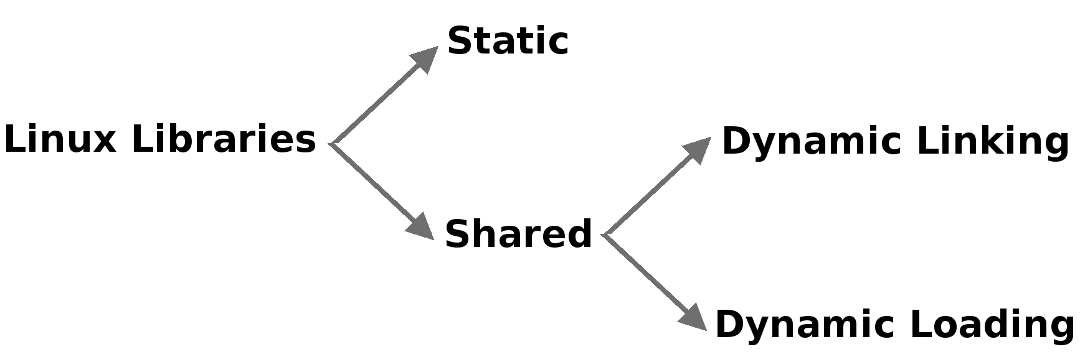
\includegraphics[width=0.71\linewidth]{os04-linux-lib}
\caption{Linux Libraries}
\end{figure}

\begin{itemize}
\item Static Libraries (embeded in the program).
\begin{itemize}
\item Self contained
\item StaticLib.a
\end{itemize}
\item Shared Libraries
\begin{itemize}
\item Dynamic Linking (run-time.so).
\item Dynamic Loading (controlled by the program, DL-API).
\end{itemize}
\end{itemize}

\end{frame}

% 8 XXXXXXXXXXXXXXXXXXXXXXXXXXXXXXXXXXXXXXXXXXXXXXXXXXXXXXXXXXXXXXXXXXXXXXXX
\section{Linux Libraries (2)}
\begin{frame}
\frametitle{Linux Libraries (2)}
\begin{itemize}
\item \texttt{putchar(char)}
\item \texttt{getpid()}
\item \texttt{getppid()}
\item \texttt{sprintf(char*, const chat*)}
\item \texttt{fflush(NULL)}
\item \texttt{MSIZE1 (10k) MSIZE2 (20k) MSIZE3 (50k) MSIZE4 (100k) MSIZE5 (1M) MSIZE6 (10M) MSIZE1}
\item \texttt{top}
\begin{itemize}
\item PID (Process Id), PPID (Parent PID), \%MEM (Memory), VIRT (Virtual Image KiB), 
	RES (Residen Size KiB), SHR (Shared Memory KiB), SWAP (Swapped Size KiB), 
	CODE (Code Size KiB), DATA (Data+Stack KiB), USED (Res+Swap Size KiB).
\item Save: \texttt{\textasciitilde{}/.toprc}
\item \texttt{top -b -n 1 -pYOUR\_PID}
\end{itemize}
\item \texttt{malloc(size\_t)}
\item \texttt{free(void*)}
\item \texttt{system(const char*)}
\end{itemize}
\end{frame}

% XXXXXXXXXXXXXXXXXXXXXXXXXXXXXXXXXXXXXXXXXXXXXXXXXXXXXXXXXXX
\section{Makefile}
\begin{frame}[fragile]
\frametitle{Makefile}
\begin{lstlisting}[basicstyle=\ttfamily\tiny]
CC=gcc
P00=00-global-variables
P01=01-local-variables
...
	
EXECS= \
        $(P00) \
        $(P01) \
...

DEMOFILES=\
	demo-file1.txt \
	demo-file2.txt \
...

all:  $(EXECS)

$(P00): $(P00).c
	$(CC) $(P00).c -o $(P00) -Xlinker -Map=$(P00).map

...

$(P04): $(P04).c
	$(CC) $(P04).c -o $(P04)
...
clean:
	rm -f ${EXECS} 
...
demo:
	bash .shsh
\end{lstlisting}
\end{frame}


% XXXXXXXXXXXXXXXXXXXXXXXXXXXXXXXXXXXXXXXXXXXXXXXXXXXXXXXXXXXXXXXXXXXXXXXXXX
\section{00-global-variables}
\begin{frame}[fragile]
\frametitle{00-global-variables}
% \begin{lstlisting}[basicstyle=\ttfamily\tiny]         % 108
% \begin{lstlisting}[basicstyle=\ttfamily\footnotesize] %  72
% \begin{lstlisting}[basicstyle=\ttfamily\small]        %  65
% \begin{lstlisting}[basicstyle=\ttfamily\large]        %  54
\begin{lstlisting}[basicstyle=\ttfamily\tiny]
/* Global Variables in Data Segment*/
char   varchr0='a';
char   varchr1='b';
char   varchr2='c';
char   varchr3='d';
char   varchr4='e';
char   varchr5='f';
char   varchr6='g';
char   varchr7='h';
VARIABLE  +++  VALUE +CHR+ + ADDRESS+
varchr0 =       0X61 = a   0x00005642d5c38038
varchr1 =       0X62 = b   0x00005642d5c38039
varchr2 =       0X63 = c   0x00005642d5c3803a
varchr3 =       0X64 = d   0x00005642d5c3803b
varchr4 =       0X65 = e   0x00005642d5c3803c
varchr5 =       0X66 = f   0x00005642d5c3803d
varchr6 =       0X67 = g   0x00005642d5c3803e
varchr7 =       0X68 = h   0x00005642d5c3803f
\end{lstlisting}

\begin{minipage}[t]{120mm}
\scalebox{0.95}{
\begin{tabular}{| c | c | c | c | c | c | c | c | c |  c  |  c  |  c  |  c  |  c  |  c  |  c  |  c |}
\hline
                    & 0 & 1 & 2 & 3 & 4 & 5 & 6 & 7 &  8  &  9  &  A  &  B  &  C  &  D  &  E  &  F  \\
\hline
0000 5642 D5C3 803X &   &   &   &   &   &   &   &   & 'a' & 'b' & 'c' & 'd' & 'e' & 'f' & 'g' & 'h' \\
\hline
\end{tabular}
}
\end{minipage}

\end{frame}

% XXXXXXXXXXXXXXXXXXXXXXXXXXXXXXXXXXXXXXXXXXXXXXXXXXXXXXXXXXXXXXXXXXXXXXXXXX
\section{Memory Map}
\begin{frame}[fragile]
\frametitle{Memory Map: 00-global-variables.map}
% \begin{lstlisting}[basicstyle=\ttfamily\tiny]         % 108
% \begin{lstlisting}[basicstyle=\ttfamily\footnotesize] %  72
% \begin{lstlisting}[basicstyle=\ttfamily\small]        %  65
% \begin{lstlisting}[basicstyle=\ttfamily\large]        %  54
\begin{lstlisting}[basicstyle=\ttfamily\tiny]
Memory Configuration (00-global-variables.map)
Archive member included to satisfy reference by file (symbol)
Memory Configuration
Name             Origin             Length             Attributes
*default*        0x0000000000000000 0xffffffffffffffff
Linker script and memory map
== TL;DR ==
.text           0x0000000000001060      0x2d1
                0x0000000000001145                main
.tdata          0x0000000000003de8        0x0
 .data          0x0000000000004038        0x8 /tmp/ccEBBZbJ.o
                0x0000000000004038                varchr0
                0x0000000000004039                varchr1
                0x000000000000403a                varchr2
                0x000000000000403b                varchr3
                0x000000000000403c                varchr4
                0x000000000000403d                varchr5
                0x000000000000403e                varchr6
                0x000000000000403f                varchr7
OUTPUT(00-global-variables elf64-x86-64)

\end{lstlisting}

\end{frame}

% XXXXXXXXXXXXXXXXXXXXXXXXXXXXXXXXXXXXXXXXXXXXXXXXXXXXXXXXXXXXXXXXXXXXXXXXXX
\section{01-local-variables}
\begin{frame}[fragile]
\frametitle{01-local-variables}

% \begin{lstlisting}[basicstyle=\ttfamily\tiny]         % 108
% \begin{lstlisting}[basicstyle=\ttfamily\footnotesize] %  72
% \begin{lstlisting}[basicstyle=\ttfamily\small]        %  65
% \begin{lstlisting}[basicstyle=\ttfamily\large]        %  54

\begin{lstlisting}[basicstyle=\ttfamily\tiny]
/* Local Variables in Stack Segment */
char   varchr0='a';
char   varchr1='b';
char   varchr2='c';
char   varchr3='d';
char   varchr4='e';
char   varchr5='f';
char   varchr6='g';
char   varchr7='h';
VARIABLE  +++  VALUE +CHR+ +++  ADDRESS +++
varchr0 =       0X61 = a   0x00007fff1e3315af
varchr1 =       0X62 = b   0x00007fff1e3315ae
varchr2 =       0X63 = c   0x00007fff1e3315ad
varchr3 =       0X64 = d   0x00007fff1e3315ac
varchr4 =       0X65 = e   0x00007fff1e3315ab
varchr5 =       0X66 = f   0x00007fff1e3315aa
varchr6 =       0X67 = g   0x00007fff1e3315a9
varchr7 =       0X68 = h   0x00007fff1e3315a8
\end{lstlisting}

\begin{minipage}[t]{120mm}

\scalebox{0.95}{

\begin{tabular}{| c | c | c | c | c | c | c | c | c |  c  |  c  |  c  |  c  |  c  |  c  |  c  |  c |}
\hline
                    & 0 & 1 & 2 & 3 & 4 & 5 & 6 & 7 &  8  &  9  &  A  &  B  &  C  &  D  &  E  &  F  \\
\hline
0000 7FFF 1E33 15AX &   &   &   &   &   &   &   &   & 'h' & 'g' & 'f' & 'e' & 'd' & 'c' & 'b' & 'a' \\
\hline
\end{tabular}
}

\end{minipage}

\end{frame}

% XXXXXXXXXXXXXXXXXXXXXXXXXXXXXXXXXXXXXXXXXXXXXXXXXXXXXXXXXXXXXXXXXXXXXXXXXX
\section{02-pointers}
\begin{frame}[fragile]
\frametitle{02-pointers (LE: Little Endian)}
% \begin{lstlisting}[basicstyle=\ttfamily\tiny]        
% \begin{lstlisting}[basicstyle=\ttfamily\footnotesize]
% \begin{lstlisting}[basicstyle=\ttfamily\small]      
% \begin{lstlisting}[basicstyle=\ttfamily\large]     
\begin{lstlisting}[basicstyle=\ttfamily\tiny]
char   varchr0='a';
char   varchr1='b';
char   varchr2='c';
char   varchr3='d';
char*  ptrchr0=&varchr0;
char*  ptrchr1=&varchr1;
char*  ptrchr2=&varchr2;
char*  ptrchr3=&varchr3;
VARIABLE  +++  VALUE +CHR+   +ADDRESS +         +POINTS TO+ 
varchr0 =       0X61 = a     0x00005650de8b0038
varchr1 =       0X62 = b     0x00005650de8b0039
varchr2 =       0X63 = c     0x00005650de8b003a
varchr3 =       0X64 = d     0x00005650de8b003b
ptrchr0 = 0x00005650de8b0038 0x00005650de8b0040     a
ptrchr1 = 0x00005650de8b0039 0x00005650de8b0048     b
ptrchr2 = 0x00005650de8b003a 0x00005650de8b0050     c
ptrchr3 = 0x00005650de8b003b 0x00005650de8b0058     d
\end{lstlisting}

\begin{minipage}[t]{120mm}
\scalebox{0.75}{
\begin{tabular}{| c | c | c | c | c | c | c | c | c |  c  |  c  |  c  |  c  |  c  |  c  |  c  |  c |}
\hline
                    &  0 &  1 &  2 &  3 &  4 &  5 &  6 &  7 &  8  &  9  &  A  &  B  &  C  &  D  &  E  &  F      \\
\hline
0000 5650 DE8B 003X &    &    &    &    &    &    &    &    & 'a' & 'b' & 'c' & 'd' &     &     &     &         \\
\hline
0000 5650 DE8B 004X & \multicolumn{8}{| c |}{0000 5650 DE8B 0038} & \multicolumn{8}{| c |}{0000 5650 DE8B 0039} \\
\hline
0000 5650 DE8B 005X & 3A & 00 & 8B & DE & 50 & 56 & 00 & 00 &  3B &  00 &  8B &  DE &  50 &  56 &  00 &  00     \\ 
\hline
\end{tabular} }
\end{minipage}

\end{frame}

% XXXXXXXXXXXXXXXXXXXXXXXXXXXXXXXXXXXXXXXXXXXXXXXXXXXXXXXXXXXXXXXXXXXXXXXXXX
\section{03-pointers-of-pointers}
\begin{frame}[fragile]
\frametitle{03-pointers-of-pointers (LE)}
% \begin{lstlisting}[basicstyle=\ttfamily\tiny] 
% \begin{lstlisting}[basicstyle=\ttfamily\footnotesize]
% \begin{lstlisting}[basicstyle=\ttfamily\small]
% \begin{lstlisting}[basicstyle=\ttfamily\large]
\begin{lstlisting}[basicstyle=\ttfamily\tiny]  
===============================================
/* Global Variables in Data Segment*/
char   varchr0='a';
char   varchr1='b';
char   varchr2='c';
char   varchr3='d';
char*  ptrchr0=&varchr0;
char*  ptrchr1=&varchr1;
char*  ptrchr2=&varchr2;
char*  ptrchr3=&varchr3;
char** ptrptr0=&ptrchr0;
char** ptrptr1=&ptrchr1;
char** ptrptr2=&ptrchr2;
char** ptrptr3=&ptrchr3;
VARIABLE  +++  VALUE +CHR+   +ADDRESS +         +POINTS TO+ 
varchr0 =       0X61 = a     0x000056200b034038
varchr1 =       0X62 = b     0x000056200b034039
varchr2 =       0X63 = c     0x000056200b03403a
varchr3 =       0X64 = d     0x000056200b03403b
ptrchr0 = 0x000056200b034038 0x000056200b034040        a
ptrchr1 = 0x000056200b034039 0x000056200b034048        b
ptrchr2 = 0x000056200b03403a 0x000056200b034050        c
ptrchr3 = 0x000056200b03403b 0x000056200b034058        d
ptrptr0 = 0x000056200b034040 0x000056200b034060 0x56200b034038
ptrptr1 = 0x000056200b034048 0x000056200b034068 0x56200b034039
ptrptr2 = 0x000056200b034050 0x000056200b034070 0x56200b03403a
ptrptr3 = 0x000056200b034058 0x000056200b034078 0x56200b03403b
==============================================================
\end{lstlisting}

\end{frame}

% XXXXXXXXXXXXXXXXXXXXXXXXXXXXXXXXXXXXXXXXXXXXXXXXXXXXXXXXXXXXXXXXXXXXXXXXXX
\begin{frame}[fragile]
\frametitle{03-pointers-of-pointers (2)}

\begin{minipage}[t]{120mm}
{\LARGE Little Endian Version A}\\[1pt]

\scalebox{0.79}{
\begin{tabular}{| c | c | c | c | c | c | c | c | c |  c  |  c  |  c  |  c  |  c  |  c  |  c  |  c |}
\hline
        &  0 &  1 &  2 &  3 &  4 &  5 &  6 &  7 &  8  &  9  &  A  &  B  &  C  &  D  &  E  &  F      \\
\hline
0000 5620 0B03 403X  &    &    &    &    &    &    &    &    & 'a' & 'b' & 'c' & 'd' &     &     &     &         \\
\hline
0000 5629 0B03 404X  & \multicolumn{8}{| c |}{0000 5620 0B03 4038} & \multicolumn{8}{| c |}{0000 5620 0B03 4039} \\
\hline
0000 5629 0B03 405X  & \multicolumn{8}{| c |}{0000 5620 0B03 403A} & \multicolumn{8}{| c |}{0000 5620 0B03 403B} \\
\hline
0000 5629 0B03 406X  & \multicolumn{8}{| c |}{0000 5620 0B03 4040} & \multicolumn{8}{| c |}{0000 5620 0B03 4048} \\
\hline
0000 5629 0B03 407X  & \multicolumn{8}{| c |}{0000 5620 0B03 4050} & \multicolumn{8}{| c |}{0000 5620 0B03 4058} \\
\hline
\end{tabular}}
\\[10mm]

{\LARGE Little Endian Version B}\\[1pt]

\scalebox{0.69}{
\begin{tabular}{| c | c | c | c | c | c | c | c | c |  c  |  c  |  c  |  c  |  c  |  c  |  c  |  c |}
\hline
                    &  0 &  1 &  2 &  3 &  4 &  5 &  6 &  7 &  8  &  9  &  A  &  B  &  C  &  D  &  E  &  F      \\
\hline
0000 5620 0B03 403X &    &    &    &    &    &    &    &    &  61 &  62 &  63 &  64 &     &     &     &         \\
\hline
0000 5620 0B03 404X & 38 & 40 & 03 & 0B & 20 & 56 & 00 & 00 &  39 &  40 &  03 &  0B &  20 &  56 &  00 &  00     \\ 
\hline
0000 5620 0B03 405X & 3A & 40 & 03 & 0B & 20 & 56 & 00 & 00 &  3B &  40 &  03 &  0B &  20 &  56 &  00 &  00     \\ 
\hline
0000 5620 0B03 406X & 40 & 40 & 03 & 0B & 20 & 56 & 00 & 00 &  48 &  40 &  03 &  0B &  20 &  56 &  00 &  00     \\ 
\hline
0000 5620 0B03 407X & 50 & 40 & 03 & 0B & 20 & 56 & 00 & 00 &  58 &  40 &  03 &  0B &  20 &  56 &  00 &  00     \\ 
\hline
\end{tabular}}
\end{minipage}

\end{frame}

% XXXXXXXXXXXXXXXXXXXXXXXXXXXXXXXXXXXXXXXXXXXXXXXXXXXXXXXXXXXXXXXXXXXXXXXXXX
\section{04-pointers-of-pointers-of-pointers}
\begin{frame}[fragile]
\frametitle{04-pointers-of-pointers-of-pointers}
% \begin{lstlisting}[basicstyle=\ttfamily\tiny]
% \begin{lstlisting}[basicstyle=\ttfamily\footnotesize]
% \begin{lstlisting}[basicstyle=\ttfamily\small]
% \begin{lstlisting}[basicstyle=\ttfamily\large]
\begin{lstlisting}[basicstyle=\ttfamily\tiny]
/* Little Endian/OLD Version        */
/* Global Variables in Data Segment */
char   varchr0='a';
char   varchr1='b';
char   varchr2='c';
char   varchr3='d';
char*  ptrchr0=&varchr0;
char*  ptrchr1=&varchr1;
char*  ptrchr2=&varchr2;
char*  ptrchr3=&varchr3;
char** ptrptr0=&ptrchr0;
char** ptrptr1=&ptrchr1;
char** ptrptr2=&ptrchr2;
char** ptrptr3=&ptrchr3;
char*** ppptr0=&ptrptr0;

VARIABLE  +++  VALUE +CHR+ +ADDRESS + +POINTS TO+ 
varchr0 =       0X61 = a    0x601038
varchr1 =       0X62 = b    0x601039
varchr2 =       0X63 = c    0x60103a
varchr3 =       0X64 = d    0x60103b
ptrchr0 =   0x601038        0x601040          a
ptrchr1 =   0x601039        0x601048          b
ptrchr2 =   0x60103a        0x601050          c
ptrchr3 =   0x60103b        0x601058          d
ptrptr0 =   0x601040        0x601060   0x601038
ptrptr1 =   0x601048        0x601068   0x601039
ptrptr2 =   0x601050        0x601070   0x60103a
ptrptr3 =   0x601058        0x601078   0x60103b
 ppptr0 =   0x601060        0x601080   0x601040
\end{lstlisting}

\end{frame}

% XXXXXXXXXXXXXXXXXXXXXXXXXXXXXXXXXXXXXXXXXXXXXXXXXXXXXXXXXXXXXXXXXXXXXXXXXX
\begin{frame}[fragile]
\frametitle{04-pointers-of-pointers-of-pointers (2)}

\begin{minipage}[t]{120mm}
\scalebox{0.75}{
\begin{tabular}{| c | c | c | c | c | c | c | c | c |  c  |  c  |  c  |  c  |  c  |  c  |  c  |  c |}
\hline
        &  0 &  1 &  2 &  3 &  4 &  5 &  6 &  7 &  8  &  9  &  A  &  B  &  C  &  D  &  E  &  F      \\
\hline
60103X  &    &    &    &    &    &    &    &    & 'a' & 'b' & 'c' & 'd' &     &     &     &         \\
\hline
60104X  & \multicolumn{8}{| c |}{601038} & \multicolumn{8}{| c |}{601039} \\
\hline
60105X  & \multicolumn{8}{| c |}{60103A} & \multicolumn{8}{| c |}{60103B} \\
\hline
60106X  & \multicolumn{8}{| c |}{601040} & \multicolumn{8}{| c |}{601048} \\
\hline
60107X  & \multicolumn{8}{| c |}{601050} & \multicolumn{8}{| c |}{601058} \\
\hline
60108X  & \multicolumn{8}{| c |}{601060} & \multicolumn{8}{| c |}{}       \\
\hline
\end{tabular}}

\begin{itemize}
\item \texttt{***ppptr0 = **ptrptr0 = *ptrchr = varchr0}
\item \texttt{ppptr0 \hspace{1pt} = [601080] = 601060}
\item \texttt{ptrptr0 = [601060] = 601040}
\item \texttt{ptrchr0 = [601040] = 601038}
\item \texttt{varchr0 = [601038] = 'a'}
\end{itemize}

\scalebox{0.60}{
\begin{tabular}{| c | c | c | c | c | c | c | c | c |  c  |  c  |  c  |  c  |  c  |  c  |  c  |  c |}
\hline
                    &  0 &  1 &  2 &  3 &  4 &  5 &  6 &  7 &  8  &  9  &  A  &  B  &  C  &  D  &  E  &  F      \\
\hline
0000 0000 0060 103X &    &    &    &    &    &    &    &    &  61 &  62 &  63 &  64 &     &     &     &         \\
\hline
0000 0000 0060 104X & 38 & 10 & 60 & 00 & 00 & 00 & 00 & 00 &  39 &  10 &  60 &  00 &  00 &  00 &  00 &  00     \\ 
\hline
0000 0000 0060 105X & 3A & 10 & 60 & 00 & 00 & 00 & 00 & 00 &  3B &  10 &  60 &  00 &  00 &  00 &  00 &  00     \\ 
\hline
0000 0000 0060 106X & 40 & 10 & 60 & 00 & 00 & 00 & 00 & 00 &  48 &  10 &  60 &  00 &  00 &  00 &  00 &  00     \\ 
\hline
0000 0000 0060 107X & 50 & 10 & 60 & 00 & 00 & 00 & 00 & 00 &  58 &  10 &  60 &  00 &  00 &  00 &  00 &  00     \\ 
\hline
0000 0000 0060 108X & 60 & 10 & 60 & 00 & 00 & 00 & 00 & 00 &     &     &     &     &     &     &     &         \\ 
\hline
\end{tabular}}
\end{minipage}

\end{frame}

% XXXXXXXXXXXXXXXXXXXXXXXXXXXXXXXXXXXXXXXXXXXXXXXXXXXXXXXXXXXXXXXXXXXXXXXXXX
\section{05-chrptr-vs-intptr}
\begin{frame}[fragile]

\frametitle{05-chrptr-vs-intptr (LE)}
% \begin{lstlisting}[basicstyle=\ttfamily\tiny]
% \begin{lstlisting}[basicstyle=\ttfamily\footnotesize]
% \begin{lstlisting}[basicstyle=\ttfamily\small]
% \begin{lstlisting}[basicstyle=\ttfamily\large]
\begin{lstlisting}[basicstyle=\ttfamily\footnotesize]
======================================
/* Global Variables in Data Segment*/
int    varint0=0x41424344;
char   varchr0='a';
char   varchr1='b';
char   varchr2='c';
char   varchr3='d';

int*   ptrint0=&varint0;
char*  ptrchr0=&varchr0;

ptrint0=(int*) &varchr2;
varint0=*ptrint0;

ptrchr0=(char*) &varint0;
varchr0=*ptrchr0;

ptrchr0++;
varchr0=*ptrchr0;
======================================
\end{lstlisting}

\end{frame}

% XXXXXXXXXXXXXXXXXXXXXXXXXXXXXXXXXXXXXXXXXXXXXXXXXXXXXXXXXXXXXXXXXXXXXXXXXX
\begin{frame}[fragile]
\frametitle{05-chrptr-vs-intptr (2)}
\begin{lstlisting}[basicstyle=\ttfamily\footnotesize]
VARIABLE  +++  VALUE +CHR+ +ADDRESS + +POINTS TO+++
varint0 = 0X41424344 = D    0x601038
varchr0 =       0X61 = a    0x60103c
varchr1 =       0X62 = b    0x60103d
varchr2 =       0X63 = c    0x60103e
varchr3 =       0X64 = d    0x60103f
ptrint0 =   0x601038        0x601048   0X41424344
ptrchr0 =   0x60103c        0x601050            a
!!! ptrint0=(int*) &varchr1;  varint0=*ptrint0; !!!
VARIABLE  +++  VALUE +CHR+ +ADDRESS + +POINTS TO+++
ptrint0 =   0x60103d       0x601048   0X65646362
varint0 = 0X65646362 = b   0x601038
\end{lstlisting}

\begin{minipage}[t]{120mm}
\scalebox{0.65}{
\begin{tabular}{| c | c | c | c | c | c | c | c | c |  c  |  c  |  c  |  c  |  c  |  c  |  c  |  c |}
\hline
                    &  0 &  1 &  2 &  3 &  4 &  5 &  6 &  7 &  8  &  9  &  A  &  B  &  C  &  D  &  E  &  F      \\
\hline
0000 0000 0060 103X &    &    &    &    &    &    &    &    &  44 &  43 &  42 &  41 &  61 &  62 &  63 &  64     \\
\hline
0000 0000 0060 104X & 65 &    &    &    &    &    &    &    &  38 &  10 &  60 &  00 &  00 &  00 &  00 &  00     \\ 
\hline
0000 0000 0060 105X & 3C & 10 & 60 & 00 & 00 & 00 & 00 & 00 &     &     &     &     &     &     &     &         \\ 
\hline
\hline
\hline
0000 0000 0060 103X &    &    &    &    &    &    &    &    &  62 &  63 &  64 &  65 &  61 &  62 &  63 &  64     \\
\hline
0000 0000 0060 104X & 65 &    &    &    &    &    &    &    &  3D &  10 &  60 &  00 &  00 &  00 &  00 &  00     \\ 
\hline
\end{tabular}}
\end{minipage}

\end{frame}

% XXXXXXXXXXXXXXXXXXXXXXXXXXXXXXXXXXXXXXXXXXXXXXXXXXXXXXXXXXXXXXXXXXXXXXXXXX
\begin{frame}[fragile]
\frametitle{05-chrptr-vs-intptr (3)}
\begin{lstlisting}[basicstyle=\ttfamily\footnotesize]
!!! ptrchr0=(char*) &varint0; varchr0=*ptrchr0; !!!
VARIABLE  +++  VALUE +CHR+ +ADDRESS + +POINTS TO+++
ptrchr0 =   0x601038       0x601050         0X62
varchr0 =       0X62 = b   0x60103c
!!!! !!!!  ptrchr0++;  varchr0=*ptrchr0;  !!!! !!!!
VARIABLE  +++  VALUE +CHR+ +ADDRESS + +POINTS TO+++
ptrchr0 =   0x601039       0x601050         0X63
varchr0 =       0X63 = c   0x60103c
\end{lstlisting}

\begin{minipage}[t]{120mm}
\scalebox{0.65}{
\begin{tabular}{| c | c | c | c | c | c | c | c | c |  c  |  c  |  c  |  c  |  c  |  c  |  c  |  c |}
\hline
                    &  0 &  1 &  2 &  3 &  4 &  5 &  6 &  7 &  8  &  9  &  A  &  B  &  C  &  D  &  E  &  F      \\
\hline
0000 0000 0060 103X &    &    &    &    &    &    &    &    &  44 &  43 &  42 &  41 &  61 &  62 &  63 &  64     \\
\hline
0000 0000 0060 104X & 65 &    &    &    &    &    &    &    &  38 &  10 &  60 &  00 &  00 &  00 &  00 &  00     \\ 
\hline
0000 0000 0060 105X & 3C & 10 & 60 & 00 & 00 & 00 & 00 & 00 &     &     &     &     &     &     &     &         \\ 
\hline
\hline
\hline
0000 0000 0060 103X &    &    &    &    &    &    &    &    &  62 &  63 &  64 &  65 &  61 &  62 &  63 &  64     \\
\hline
0000 0000 0060 104X & 65 &    &    &    &    &    &    &    &  3D &  10 &  60 &  00 &  00 &  00 &  00 &  00     \\ 
\hline
\hline
\hline
0000 0000 0060 103X &    &    &    &    &    &    &    &    &  62 &  63 &  64 &  65 &  62 &  62 &  63 &  64     \\
\hline
0000 0000 0060 105X & 38 & 10 & 60 & 00 & 00 & 00 & 00 & 00 &     &     &     &     &     &     &     &         \\ 
\hline
\hline
\hline
\hline
0000 0000 0060 103X  &    &    &    &    &    &    &    &    &  62 &  63 &  64 &  65 &  63 &  62 &  63 &  64     \\
\hline
0000 0000 0060 105X  & 39 & 10 & 60 & 00 & 00 & 00 & 00 & 00 &     &     &     &     &     &     &     &         \\ 
\hline
\end{tabular}}
\end{minipage}

\end{frame}

% XXXXXXXXXXXXXXXXXXXXXXXXXXXXXXXXXXXXXXXXXXXXXXXXXXXXXXXXXXXXXXXXXXXXXXXXXX
\section{06-pointer-address}
\begin{frame}[fragile]
\frametitle{06-pointer-address (LE)}
% \begin{lstlisting}[basicstyle=\ttfamily\small]
\begin{lstlisting}[basicstyle=\ttfamily\footnotesize]
unsigned char   varchr0='a';
unsigned char*  ptrchr0=&varchr0;
unsigned char*  ptrcopy=(char *) &ptrchr0;

VARIABLE  +++  VALUE +++ +CHR+ +++ ADDRESS  +++ +PTS TO+
varchr0 =           0X61 = a    0x7ffe7bb7369f
ptrchr0 = 0x7ffe7bb7369f        0x7ffe7bb73690     0X61

!!! !!!!! ptrcopy++; ptrcopy++; ptrcopy++; ... !!!!! !!!
ptrcopy = 0x7ffe7bb73690        0x7ffe7bb73688     0X9F
ptrcopy = 0x7ffe7bb73691        0x7ffe7bb73688     0X36
ptrcopy = 0x7ffe7bb73692        0x7ffe7bb73688     0XB7
ptrcopy = 0x7ffe7bb73693        0x7ffe7bb73688     0X7B
ptrcopy = 0x7ffe7bb73694        0x7ffe7bb73688     0XFE
ptrcopy = 0x7ffe7bb73695        0x7ffe7bb73688     0X7F
ptrcopy = 0x7ffe7bb73696        0x7ffe7bb73688       00
ptrcopy = 0x7ffe7bb73697        0x7ffe7bb73688       00
\end{lstlisting}

\end{frame}

% XXXXXXXXXXXXXXXXXXXXXXXXXXXXXXXXXXXXXXXXXXXXXXXXXXXXXXXXXXXXXXXXXXXXXXXXXX

\begin{frame}[fragile]
\frametitle{06-pointer-address (2)}
\begin{lstlisting}[basicstyle=\ttfamily\tiny]
!!! !!!!! ptrcopy++; ptrcopy++; ptrcopy++; ... !!!!! !!!
VARIABLE  +++  VALUE +++ +CHR+ +++ ADDRESS  +++ +PTS TO+
ptrchr0 = 0x7ffe7bb7369f        0x7ffe7bb73690     0X61
ptrcopy = 0x7ffe7bb73690        0x7ffe7bb73688     0X9F
ptrcopy = 0x7ffe7bb73691        0x7ffe7bb73688     0X36
ptrcopy = 0x7ffe7bb73692        0x7ffe7bb73688     0XB7
ptrcopy = 0x7ffe7bb73693        0x7ffe7bb73688     0X7B
ptrcopy = 0x7ffe7bb73694        0x7ffe7bb73688     0XFE
ptrcopy = 0x7ffe7bb73695        0x7ffe7bb73688     0X7F
ptrcopy = 0x7ffe7bb73696        0x7ffe7bb73688       00
ptrcopy = 0x7ffe7bb73697        0x7ffe7bb73688       00
\end{lstlisting}

\begin{minipage}[t]{120mm}
\scalebox{0.65}{
\begin{tabular}{| c | c | c | c | c | c | c | c | c |  c  |  c  |  c  |  c  |  c  |  c  |  c  |  c |}
\hline
                    &  0 &  1 &  2 &  3 &  4 &  5 &  6 &  7 &  8 &  9 &  A &  B &  C &  D &  E &  F \\
\hline
0000 7FFE 7BB7 368X  &    &    &    &    &    &    &    &    & 90 & 36 & B7 & 7B & FE & 7F & 00 & 00 \\
0000 7FFE 7BB7 369X  & 9F & 36 & B7 & 7B & FE & 7F & 00 & 00 &    &    &    &    &    &    &    & 61 \\
\hline
\hline
\hline
0000 7FFE 7BB7 368X  &    &    &    &    &    &    &    &    & 91 & 36 & B7 & 7B & FE & 7F & 00 & 00 \\
\hline
\hline
0000 7FFE 7BB7 368X  &    &    &    &    &    &    &    &    & 92 & 36 & B7 & 7B & FE & 7F & 00 & 00 \\
\hline
\hline
0000 7FFE 7BB7 368X  &    &    &    &    &    &    &    &    & 93 & 36 & B7 & 7B & FE & 7F & 00 & 00 \\
\hline
\hline
0000 7FFE 7BB7 368X  &    &    &    &    &    &    &    &    & 94 & 36 & B7 & 7B & FE & 7F & 00 & 00 \\
\hline
\hline
0000 7FFE 7BB7 368X  &    &    &    &    &    &    &    &    & 95 & 36 & B7 & 7B & FE & 7F & 00 & 00 \\
\hline
\hline
0000 7FFE 7BB7 368X  &    &    &    &    &    &    &    &    & 96 & 36 & B7 & 7B & FE & 7F & 00 & 00 \\
\hline
\hline
0000 7FFE 7BB7 368X  &    &    &    &    &    &    &    &    & 97 & 36 & B7 & 7B & FE & 7F & 00 & 00 \\
\hline
\end{tabular}}
\end{minipage}

\end{frame}

% XXXXXXXXXXXXXXXXXXXXXXXXXXXXXXXXXXXXXXXXXXXXXXXXXXXXXXXXXXX
\section{07-addresses}
\begin{frame}[fragile]
\frametitle{07-addresses (LE)}
% \begin{lstlisting}[basicstyle=\ttfamily\small]
\begin{lstlisting}[basicstyle=\ttfamily\footnotesize]
unsigned int  glInt1 = 0x41;
unsigned int  glInt2 = 0x42;
unsigned int  glInt3 = 0x43;
unsigned int  glInt4 = 0x44;
unsigned int  glInt5 = 0x45;
unsigned int* heapArray[] = {&glInt1, &glInt2, &glInt3, &glInt4, &glInt5};

Variable Name     Address   Size(S)/Value(V)
============================================
glInt1            0x601060        0X41 (V) 
glInt2            0x601064        0X42 (V) 
glInt3            0x601068        0X43 (V) 
glInt4            0x60106c        0X44 (V) 
heapArray---      0x601080    0X601060 (V) 
heapArray[0]      0x601080    0X601060 (V) 
heapArray[1]      0x601088    0X601064 (V) 
heapArray[2]      0x601090    0X601068 (V) 
heapArray[3]      0x601098    0X60106C (V) 
heapArray[4]      0x6010a0    0X601070 (V)
\end{lstlisting}

\end{frame}

% XXXXXXXXXXXXXXXXXXXXXXXXXXXXXXXXXXXXXXXXXXXXXXXXXXXXXXXXXXX
\begin{frame}[fragile]
\frametitle{07-addresses (2)}
% \begin{lstlisting}[basicstyle=\ttfamily\small]
\begin{lstlisting}[basicstyle=\ttfamily\footnotesize]
#define ALLOC0  0x4BD8
#define ALLOC1  0xFF8
#define ALLOC2  0x18
#define ALLOC3  0x19
#define ALLOC4  1
heapArray[0]=malloc(ALLOC0);
heapArray[1]=malloc(ALLOC1);
heapArray[2]=malloc(ALLOC2);
heapArray[3]=malloc(ALLOC3);
heapArray[4]=malloc(ALLOC4);

Variable Name     Address   Size(S)/Value(V)
============================================
heapArray---      0x601080   0X23CF420 (V) 
heapArray[0]      0x601080   0X23CF420 (V) 
heapArray[1]      0x601088   0X23D4000 (V) 
heapArray[2]      0x601090   0X23D5000 (V) 
heapArray[3]      0x601098   0X23D5020 (V) 
heapArray[4]      0x6010a0   0X23D5050 (V)
\end{lstlisting}

\end{frame}

% XXXXXXXXXXXXXXXXXXXXXXXXXXXXXXXXXXXXXXXXXXXXXXXXXXXXXXXXXXX
\begin{frame}[fragile]
\frametitle{07-addresses (3)}
% \begin{lstlisting}[basicstyle=\ttfamily\small]
\begin{lstlisting}[basicstyle=\ttfamily\footnotesize]

long printVariable(char* varName, void* varValue, long endAddr) { ... }
long printHeapArray(int mode) { ... }
long demoMalloc(int mode) { ... }
long tripleLoop(int mode) { ... }
void main(void)           { ... }

Variable Name     Address   Size(S)/Value(V)
============================================
printf            0x400480
malloc            0x400490
printVariable     0x400596        0XBE (S)
printHeapArray    0x400654        0XA3 (S)
demoMalloc        0x4006f7        0X7E (S)
tripleLoop        0x400775        0XFC (S)
main              0x400871       0X148 (S)

\end{lstlisting}
\end{frame}

% XXXXXXXXXXXXXXXXXXXXXXXXXXXXXXXXXXXXXXXXXXXXXXXXXXXXXXXXXXX
\begin{frame}[fragile]
\frametitle{07-addresses (3)}
% \begin{lstlisting}[basicstyle=\ttfamily\small]
\begin{lstlisting}[basicstyle=\ttfamily\tiny]

####################################################################################################

Memory Configuration
                0x0000000000400238       (SEGMENT-START ("text-segment", 0x400000) + SIZEOF-HEADERS)

 .plt           0x0000000000400460       0x40 /usr/lib/gcc/.../x86-64-linux-gnu/crt1.o
                0x0000000000400470                puts@@GLIBC\_2.2.5
                0x0000000000400480                printf@@GLIBC\_2.2.5
                0x0000000000400490                malloc@@GLIBC\_2.2.5

.text           0x00000000004004a0      0x592
 .text          0x0000000000400596      0x41d /tmp/ccU78N7D.o
                0x0000000000400596                printVariable
                0x0000000000400654                printHeapArray
                0x00000000004006f7                demoMalloc
                0x0000000000400775                tripleLoop
                0x0000000000400871                main

 .data          0x0000000000601060       0x48 /tmp/ccU78N7D.o
                0x0000000000601060                glInt1
                0x0000000000601064                glInt2
                0x0000000000601068                glInt3
                0x000000000060106c                glInt4
                0x0000000000601070                glInt5
                0x0000000000601080                heapArray

####################################################################################################

\end{lstlisting}
\end{frame}

% XXXXXXXXXXXXXXXXXXXXXXXXXXXXXXXXXXXXXXXXXXXXXXXXXXXXXXXXXXX
\section{08-passing-parameters}
\begin{frame}[fragile]
\frametitle{08-passing-parameters}
% \begin{lstlisting}[basicstyle=\ttfamily\small]
\begin{lstlisting}[basicstyle=\ttfamily\tiny]
#define NOP()    __asm__("nop")  /* No Operation inline gcc ASM *** */
#include <stdio.h>
int  varInt1   = 0x01;
int  varInt2   = 0x02;
int* ptrInt1   = &varInt1;
int* ptrInt2   = &varInt2;
void function1(void) {
   NOP();
}
void function2(int iif2) {
   printf("function2:     iif2 = %d\n", ++iif2);
}
void function3(int* iif3) {
   printf("function3:     iif3 = %d\n", ++(*iif3));
}
int  function4(void) {
   NOP();
}
int* function5(void) {
   NOP();
}
void main(void) {                                   // main-1:    *ptrInt1 = 1
   function1();                                     // function2:     iif2 = 2
   printf("main-1:    *ptrInt1 = %d\n", *ptrInt1);  // main-2:    *ptrInt1 = 1
   function2(*ptrInt1);                             // main-3:     varInt1 = 1
   printf("main-2:    *ptrInt1 = %d\n", *ptrInt1);  // function3:     iif3 = 2
   printf("main-3:     varInt1 = %d\n",  varInt1);  // main-4:     varInt1 = 2
   function3(&varInt1);
   printf("main-4:     varInt1 = %d\n",  varInt1);
}

\end{lstlisting}
\end{frame}

% XXXXXXXXXXXXXXXXXXXXXXXXXXXXXXXXXXXXXXXXXXXXXXXXXXXXXXXXXXX
\section{09-struct}
\begin{frame}[fragile]
\frametitle{09-struct}
\begin{lstlisting}[basicstyle=\ttfamily\tiny]

#include <stdio.h>
typedef struct {
   char* nama;
   int   umur;
   int   semester;
   char* NIM;
} student;

void printStruct(student* ss) {
   printf("%-10s %11s %3d %2d\n", ss->nama, ss->NIM, ss->umur, ss->semester);
}

student global;
void init(void) {
   global.nama     = "Burhan";
   global.NIM      = "1205000003";
   global.umur     = 10;
   global.semester = 2;
}

void main(void) {
   student mhs = {"Ali", 12, 1, "1205000001"};
   printStruct(&mhs);
   init();
   printStruct(&global);
}
==============================
Ali         1205000001  12  1
Burhan      1205000003  10  2

\end{lstlisting}
\end{frame}

% XXXXXXXXXXXXXXXXXXXXXXXXXXXXXXXXXXXXXXXXXXXXXXXXXXXXXXXXXXXXXXXXXXXXXXXXXX

\end{document}

